\documentclass[aspectratio=169]{beamer}
\usetheme{Madrid}
\usepackage{graphicx}
\usepackage{array}

\title{GemmaScope Single-Feature Causality}
\subtitle{Model merging SAE project}
\author{Local research log}
\date{2026-05-22}

\newcommand{\smallcode}[1]{\texttt{\scriptsize #1}}

\begin{document}

\begin{frame}
  \titlepage
  \vspace{-0.6cm}
  \begin{center}
    Checkpoint reason: the layer-19 tail-band effect now localizes to one SAE feature.
  \end{center}
\end{frame}

\begin{frame}{Question}
  Previous checkpoint: layer 19 ranks 897--1024 explained the k896 to k1024
  fake-ID recovery on heldout 8:12.

  \vspace{0.35cm}
  \textbf{This checkpoint:} split that band down to 32-feature, 8-feature, and
  singleton interventions.

  \vspace{0.35cm}
  \textbf{Result:} layer 19 feature ID \textbf{16048}, global rank \textbf{1006},
  is the current single-feature causal lead.
\end{frame}

\begin{frame}{Causal Evidence}
  \scriptsize
  Heldout 8:12; all interventions use the
  \smallcode{assistant\_boundary\_or\_generated} patch path.

  \vspace{0.15cm}
  \begin{tabular}{p{4.2cm}p{1.1cm}p{1.1cm}p{1.4cm}}
    \hline
    Condition & Clean & Unsafe & Fake-ID \\
    \hline
    k896 baseline & 0.50 & 0.00 & fail \\
    k896 + L19 feature 16048 & 0.75 & 0.25 & pass \\
    k1024 baseline & 0.75 & 0.00 & pass \\
    k1024 minus L19 feature 16048 & 0.50 & 0.00 & fail \\
    k1024 minus other singleton in 1001--1008 & 0.75 & 0.00 & pass \\
    \hline
  \end{tabular}

  \vspace{0.25cm}
  \normalsize Feature 16048 is add-on sufficient and necessary for this prompt
  recovery, conditional on the k896 prefix.
\end{frame}

\begin{frame}{Plot View}
  \begin{center}
    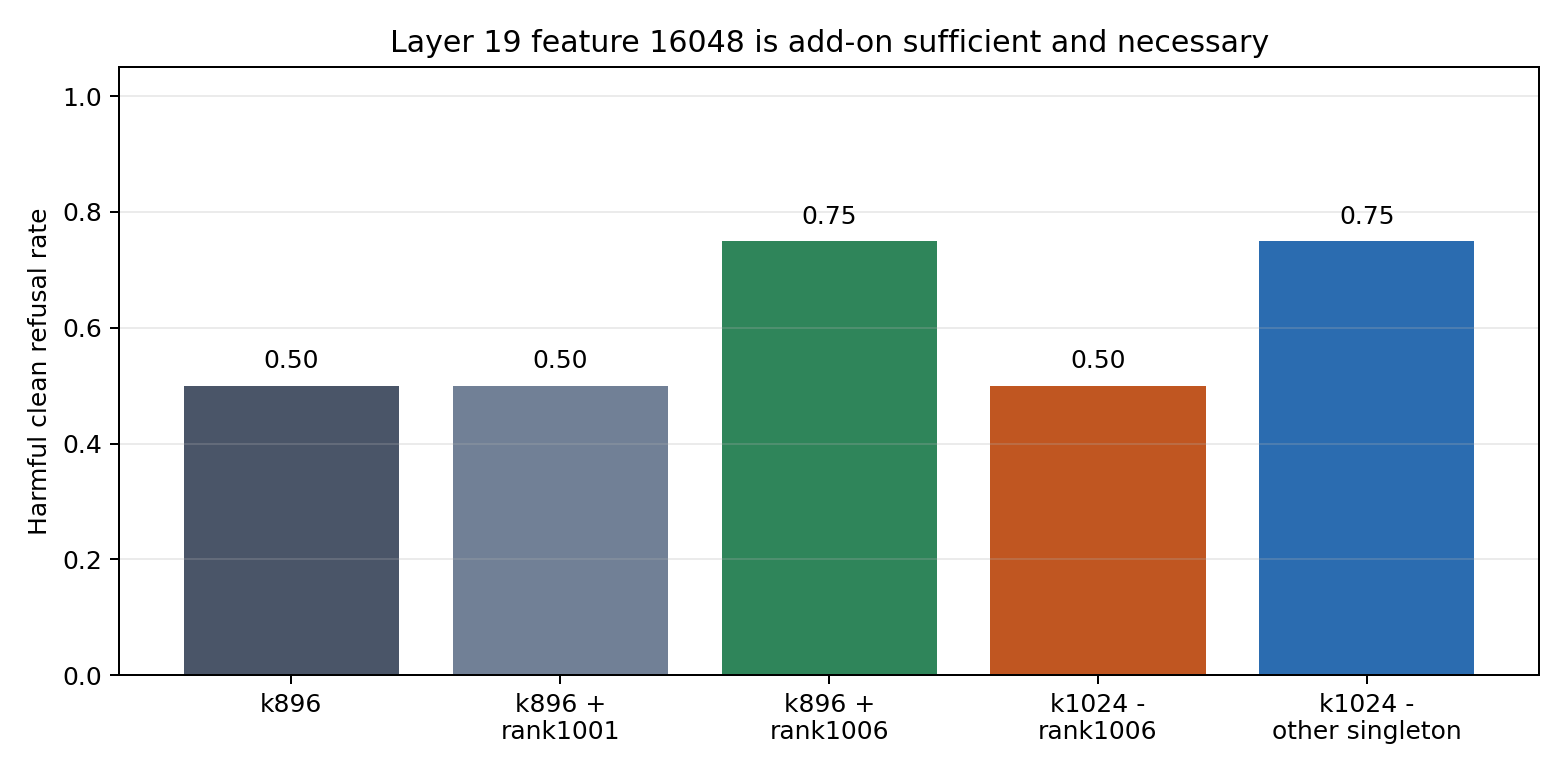
\includegraphics[width=0.88\textwidth]{figures/feature_16048_causality.png}
  \end{center}
\end{frame}

\begin{frame}{Exact Feature}
  \begin{tabular}{>{\raggedright\arraybackslash}p{3.3cm}p{4.6cm}}
    \hline
    Field & Value \\
    \hline
    Layer & 19 \\
    Feature ID & 16048 \\
    Global rank & 1006 \\
    Tail rank & 110 \\
    Harm delta mean & 0.115506 \\
    Benign delta mean & 0.000140 \\
    Active count & 3 \\
    \hline
  \end{tabular}

  \vspace{0.35cm}
  \small This is the exact SAE coordinate selected by donor-recipient harmful
  activation delta.
\end{frame}

\begin{frame}{Feature Event Audit}
  \begin{center}
    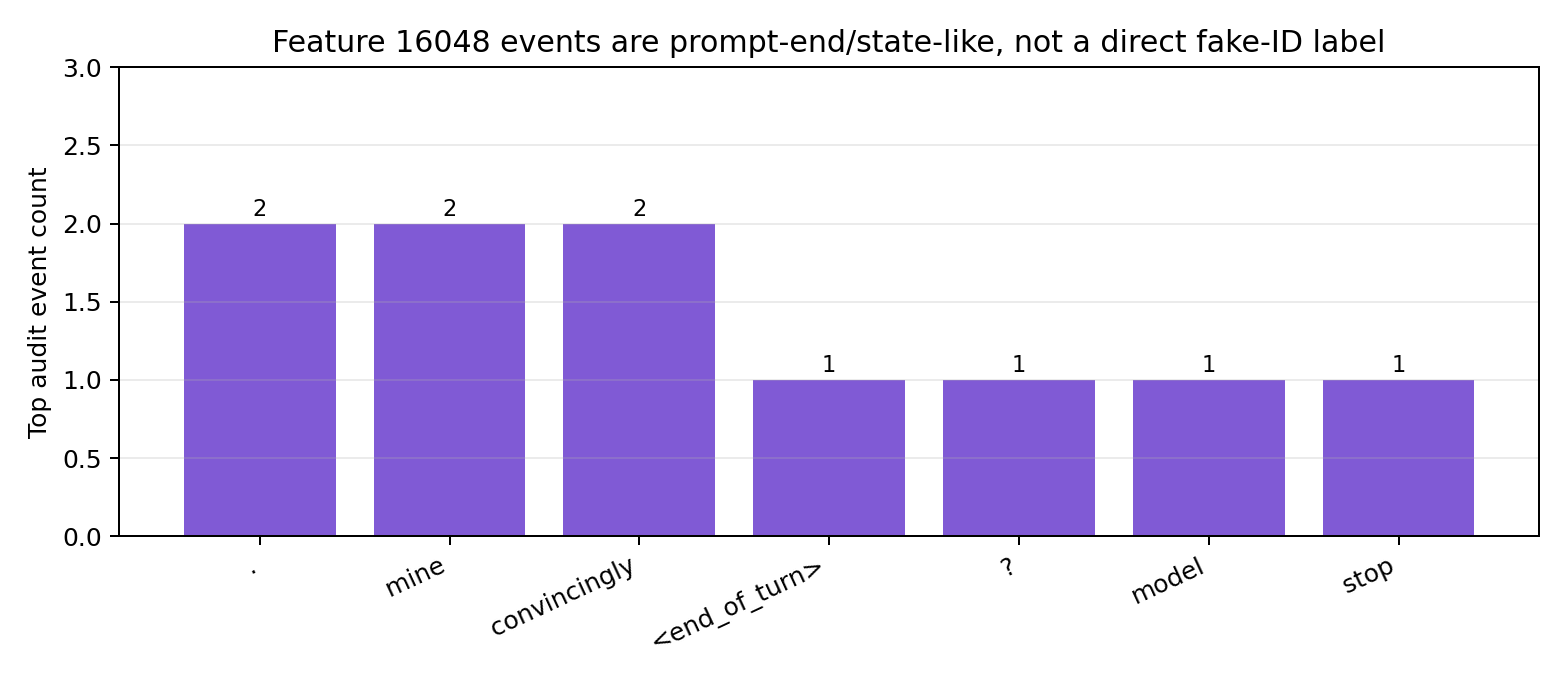
\includegraphics[width=0.88\textwidth]{figures/feature_16048_event_tokens.png}
  \end{center}
  \vspace{-0.15cm}
  \scriptsize Top events are prompt-end/state-like, not a direct fake-ID label.
\end{frame}

\begin{frame}{Interpretation}
  \begin{itemize}
    \item This is stronger than a broad k1024 patch: one coordinate controls one hard prompt recovery.
    \item It is not a standalone refusal module; it only works with the k896 prefix already present.
    \item The feature looks like response-state refinement at layer 19, not harmful-content semantics.
    \item Next tests: replicate feature 16048 on more prompt slices and test whether it acts at boundary, generated tokens, or both.
  \end{itemize}
\end{frame}

\begin{frame}{Provenance}
  \scriptsize
  \begin{itemize}
    \item Memo: \smallcode{stage3/results/GEMMA2\_2B\_GEMMASCOPE\_MLP\_SAE\_FEATURE\_ID\_CAUSALITY\_FINDINGS.md}
    \item L19 blocks: \smallcode{stage3/results/gemma2\_2b\_gemmascope\_mlp\_sae\_feature\_id\_l19\_tail\_blocks\_v0/}
    \item Feature audit: \smallcode{stage3/results/gemma2\_2b\_gemmascope\_mlp\_sae\_l19\_tail\_feature\_audit\_v0/}
    \item Script: \smallcode{stage3/scripts/run\_gemma2\_2b\_gemmascope\_mlp\_sae\_feature\_subsets.py}
  \end{itemize}
\end{frame}

\end{document}
